
% This LaTeX was auto-generated from an M-file by MATLAB.
% To make changes, update the M-file and republish this document.

\documentclass{article}
\usepackage{graphicx}
\usepackage{color}

\sloppy
\definecolor{lightgray}{gray}{0.5}
\setlength{\parindent}{0pt}

\begin{document}

    
    
\section*{Exercise 7}

\begin{par}
Compare two different iterative square-root functions.
\end{par} \vspace{1em}
\begin{par}
Given an input $x[n] = \alpha\mu[n]$, where $\alpha$ is the number whose square root is desired.  For this system $\alpha$ must be between 0 and 1.
\end{par} \vspace{1em}

\subsection*{Contents}

\begin{itemize}
\setlength{\itemsep}{-1ex}
   \item User inputs
   \item Generate Working Values
   \item Calculate the square roots
   \item Plot
   \item Efficiency Comparison
\end{itemize}


\subsection*{User inputs}

\begin{verbatim}
% Provide a seed value y[-1], for the calculations
yInit = 0.5;
% Provide $\alpha$, the number whose square root we are calculating
alpha = .9;
% Provide the number of iterations to calculate
iterations = 100;
\end{verbatim}


\subsection*{Generate Working Values}

\begin{verbatim}
x = alpha * ones(1,iterations);
\end{verbatim}


\subsection*{Calculate the square roots}

\begin{verbatim}
Output7a = Exercise7a(x,yInit);
Output7b = Exercise7b(x,yInit);
\end{verbatim}


\subsection*{Plot}

\begin{verbatim}
OutputFig = figure;
subplot(2,1,1);
stem(Output7a)
title('Output of $\displaystyle y[n] = \frac{1}{2} \left(y[n-1] + \frac{x[n]}{y[n-1]}\right)$',...
    'interpreter','latex')

subplot(2,1,2);
stem(Output7b)
title('Output of $\displaystyle y[n] = x[n] - y^2[n-1] + y[n-1]$', ...
    'interpreter','latex')
\end{verbatim}

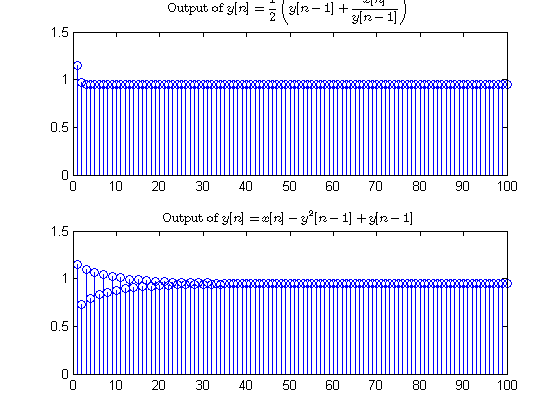
\includegraphics [width=4in]{Exercise7_01.png}


\subsection*{Efficiency Comparison}

\begin{par}
Evaluate how many iterations each function takes to get within 4 decimal places of accuracy over a range of inputs.
\end{par} \vspace{1em}
\begin{verbatim}
% Check 100 input values between 0 and 1, for statistics purposes.
inputs = linspace(0,1,1000);

outputs = zeros(2,size(inputs,2));

% I'm going to go loop-heavy here because it's non-critical code

for iter = 1:size(inputs,2)
    x = inputs(iter) * ones(1,iterations);

    compare = sqrt(x(1));

    Output7a = Exercise7a(x,yInit);
    Output7b = Exercise7b(x,yInit);

    for n = 1:size(Output7a,2)
        E = abs(compare - Output7a(n));
        if E < 0.0001
            outputs(1,iter) = n;
            break
        end
    end

    for n = 1:size(Output7a,2)
        E = abs(compare - Output7b(n));
        if E < 0.0001
            outputs(2,iter) = n;
            break
        end
    end
end

% Display the average of all of the iterations required over a range of
% input values.
averages = mean(outputs,2)
\end{verbatim}

        \color{lightgray} \begin{verbatim}
averages =

    3.0240
   15.6700

\end{verbatim} \color{black}
    


\end{document}
    
